\documentclass[a4paper,12pt]{article}
\usepackage[utf8]{inputenc}
\usepackage[italian]{babel}
\usepackage{amsfonts}
\usepackage{listings}
\usepackage{xcolor}
\usepackage{booktabs}
\usepackage{graphicx}
\usepackage{float}

\title{Relazione sul Funzionamento Interno di Python}
\author{Appunti di Programmazione}
\date{\today}

\begin{document}
\tableofcontents
\newpage

\maketitle

\section{Introduzione a Python}
Python è un linguaggio di programmazione ad alto livello, interpretato e multi-paradigma. A differenza dei linguaggi puramente compilati (come il C), Python utilizza un sistema ibrido che garantisce portabilità e flessibilità.

\section{Il Flusso di Esecuzione}
Il passaggio dal codice sorgente all'esecuzione sulla CPU non è diretto, ma attraversa diverse fasi cruciali:

\begin{figure}[H]
    \centering
    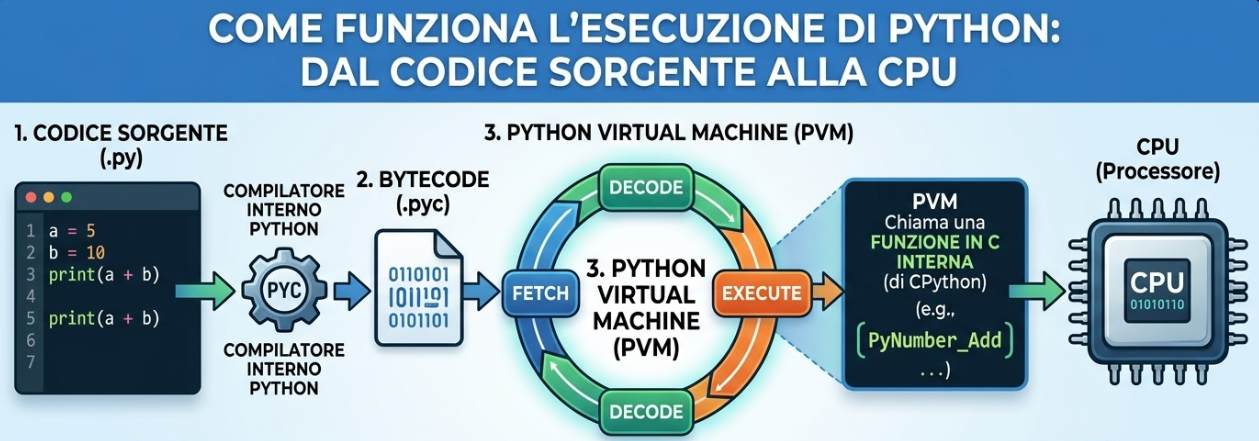
\includegraphics[width=0.8\linewidth]{Immagini/ExecutionFlux.png}
    \caption{Funzionamento python con PVM}
\end{figure}

\begin{itemize}
    \item \textbf{Compilazione in Bytecode}                     Quando un file \texttt{.py} viene eseguito, l'interprete (solitamente CPython) lo traduce in un formato intermedio chiamato \textbf{Bytecode}. Questo codice non è leggibile dall'uomo né direttamente dalla CPU, ma è ottimizzato per l'interprete. I file risultanti hanno spesso estensione \texttt{.pyc}.
    \item \textbf{La python Virtual Machine (PVM)}              La PVM è il cuore del runtime di Python. Si tratta di un software che emula un microprocessore e agisce come strato di astrazione tra il Bytecode e l'hardware sottostante.
    \item \textbf{Il Meccanismo Interno: L'Interpreter Loop}    La PVM opera attraverso un ciclo continuo di \textit{Fetch-Decode-Execute}. Il dettaglio del funzionamento è il seguente:
            \begin{enumerate}
                \item \textbf{Fetch:} La PVM preleva la successiva istruzione di Bytecode.
                \item \textbf{Decode:} L'istruzione viene identificata (es. \texttt{BINARY\_ADD}).
                \item \textbf{Execute:} La PVM richiama una funzione interna scritta in \textbf{linguaggio C} (le cosiddette \textit{C-API} di CPython).
                \item \textbf{Linguaggio Macchina:} La funzione C, essendo già compilata, viene eseguita direttamente dal processore come sequenza di istruzioni binarie.
            \end{enumerate}
\end{itemize}




\subsection{Confronto tra C e Python}

\begin{figure}[H]
    \centering
    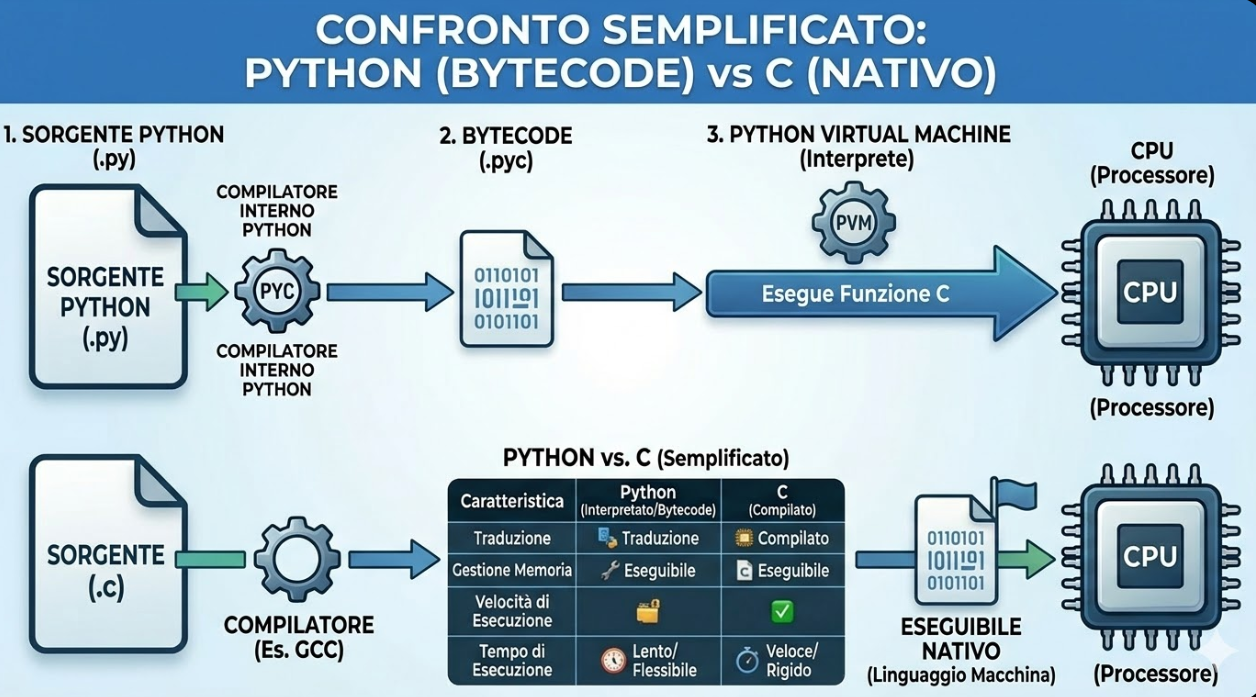
\includegraphics[width=0.8\linewidth]{Immagini/CvsPython.png}
    \caption{Confronto tra C e Python}
\end{figure}

\begin{table}[H]
\centering
\begin{tabular}{@{}lll@{}}
\toprule
\textbf{Caratteristica} & \textbf{Linguaggio C} & \textbf{Python} \\ \midrule
\textbf{Traduzione} & Compilazione statica & Compilazione JIT/Bytecode \\
\textbf{Eseguibile} & Binario nativo (OS-specific) & Bytecode (Universale) \\
\textbf{Astrazione} & Bassa (vicino all'hardware) & Alta (astrazione totale) \\
\textbf{Gestione Memoria} & Manuale (\texttt{malloc}/\texttt{free}) & Automatica (Garbage Collector) \\ \bottomrule
\end{tabular}
\caption{Differenze architetturali principali.}
\end{table}

\subsection{Esempio}

Supponiamo di avere il seguente codice python:
\begin{figure}[H]
    \centering
    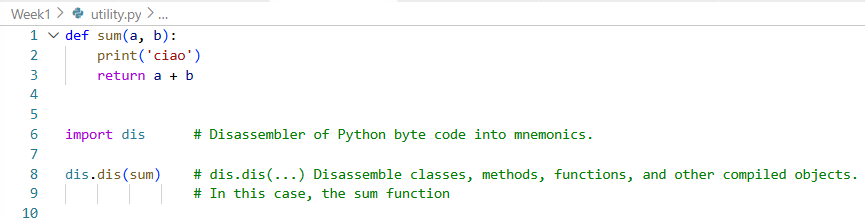
\includegraphics[width = 0.7\linewidth]{Immagini/Utility.png}
\end{figure}

Il modulo \textit{dis} è il disassemblatore.
Il suo compito è prendere il codice Python (che è scritto in un linguaggio comprensibile agli umani) e mostrarti le istruzioni a basso livello
che la Python Virtual Machine (PVM) esegue effettivamente "sotto il cofano".

L'output è il seguente:

\begin{figure}[H]
    \centering
    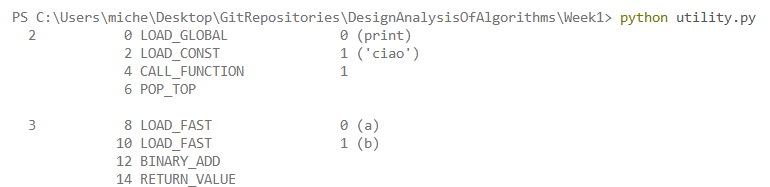
\includegraphics[width=0.7\linewidth]{Immagini/outputUtility.png}
\end{figure}

Il blocco \texttt{print('ciao')} (Righe 0-6)
Qui Python sta preparando una chiamata a funzione:
\begin{itemize}
    \item \textbf{LOAD\_GLOBAL 0 (print)}: Python deve andare a cercare la funzione print. Dato che non è definita dentro la tua funzione sum, la cerca nello spazio "Globale" (o nei built-ins).
    \item \textbf{LOAD\_CONST 1 ('ciao')}: Carica l'argomento da passare alla funzione.
    \item \textbf{CALL\_FUNCTION 1: Dice alla PVM}: "\textit{Prendi la funzione che hai caricato, passale 1 argomento e avviala}". Qui la PVM sospende per un attimo sum e va a eseguire il codice C di print.
    \item \textbf{POP\_TOP}: Questa è fondamentale. La funzione print restituisce sempre None, che viene messo sullo stack. Dato che non stai salvando il risultato di print in una variabile (es. non hai scritto x = print('ciao')),
    Python "pulisce" lo stack eliminando quel None.
\end{itemize}

Il blocco \texttt{return a + b} (Righe 8-14)
\begin{itemize}
    \item \textbf{LOAD\_FAST 0 (a) e 1 (b)}: Python carica i valori dei parametri locali. L'uso di \textit{FAST} indica che l'accesso avviene tramite un indice in un array locale, rendendolo molto più rapido rispetto alla ricerca in un dizionario globale.
    \item \textbf{BINARY\_ADD}: L'istruzione preleva i due valori dallo stack e invoca la routine C corrispondente per eseguire l'addizione. Il risultato viene poi riposto in cima allo stack.
    \item \textbf{RETURN\_VALUE}: Conclude l'esecuzione della funzione restituendo al chiamante l'elemento attualmente presente in cima allo stack.
\end{itemize}





\subsection{Conclusione}
Sebbene l'interposizione della PVM renda Python intrinsecamente più lento del C, questo approccio permette una gestione della memoria semplificata, una portabilità cross-platform immediata e una velocità di sviluppo superiore, delegando le operazioni critiche a routine interne pre-ottimizzate in C.






\newpage
\section{Trees Hierarchy}

\begin{figure}[H]
    \centering
    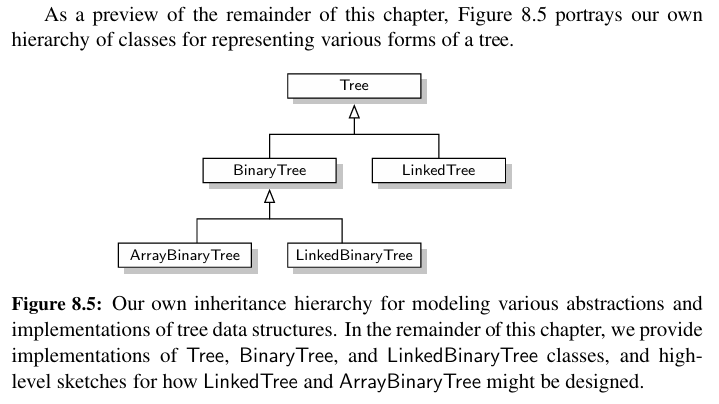
\includegraphics[width=0.7\linewidth]{Immagini/TreesHierarchy.png}
\end{figure}

\subsection{General Tree}

\begin{figure}[H]
    \centering
    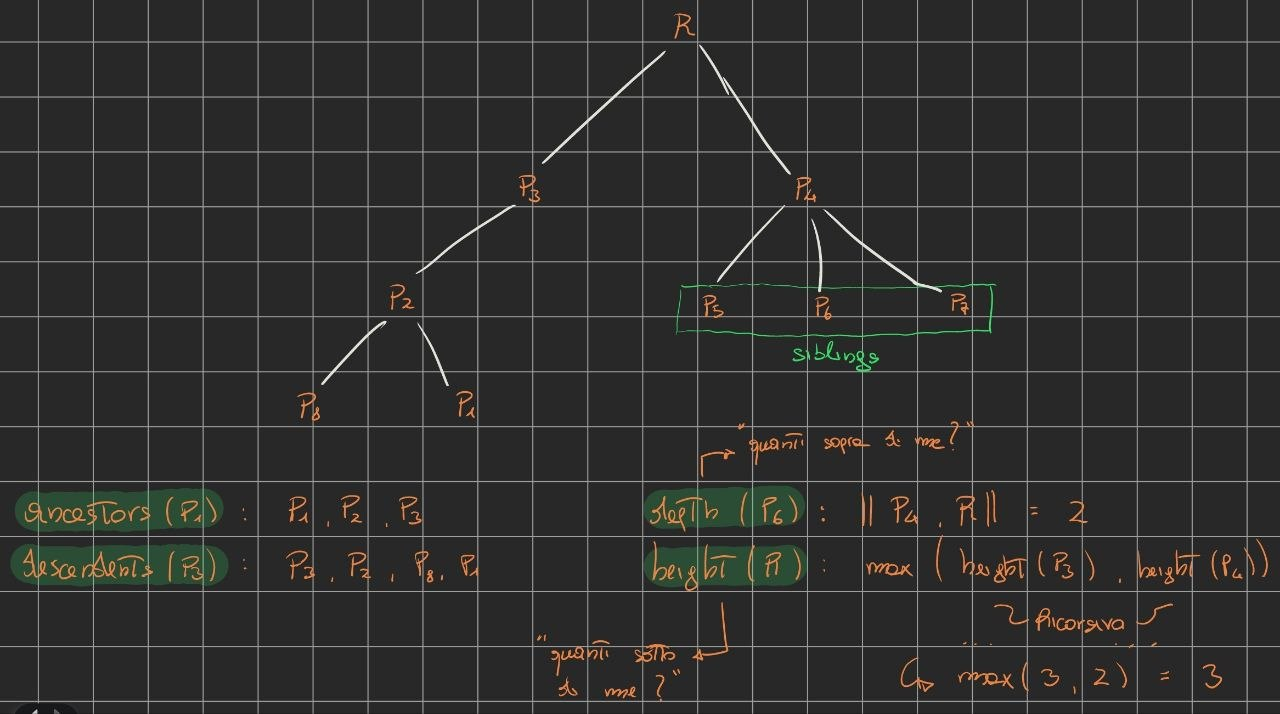
\includegraphics[width=0.7\linewidth]{Immagini/GeneralTree.png}
\end{figure}

\begin{itemize}
    \item Ogni nodo, escluso il nodo in alto (Radice), ha un padre e un numero arbitrario di figli.
    \item Due nodi che sono figli dello stesso padre sono frtelli;
    \item Un nodo è una foglia se non ha figli.
    \item Un nodo è interno se ha almeno un figlio.
    \item un nodo \textit{v} è un \textbf{antenato} di un nodo \textit{u} se \textit{u = v} o
          \textit{u} è un antenato del padre di \textit{v}.
    \item Un nodo \textit{v} è un \textbf{descendente} di un nodo \textit{u} se u è un antenato di \textit{v}.
    \item Un \textbf{edge} è una coppia di nodi \textit{(u, v)} tale che \textit{u} è il padre di \textit{v} o viceversa.
    \item Un \textbf{path} è una sequenza di nodi tali che qualsiasi coppia di nodi consecutivi è un \textbf{edge}.
\end{itemize}

\subsubsection{General Tree - Abstract Data Type}

\begin{figure}[H]
    \centering
    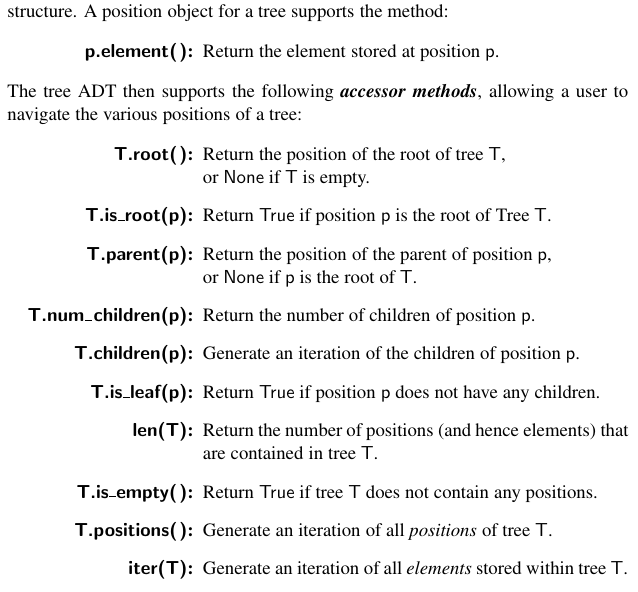
\includegraphics[width=0.7\linewidth]{Immagini/ADT_Tree.png}
\end{figure}


\subsection{Binary Tree}
\begin{figure}[H]
    \centering
    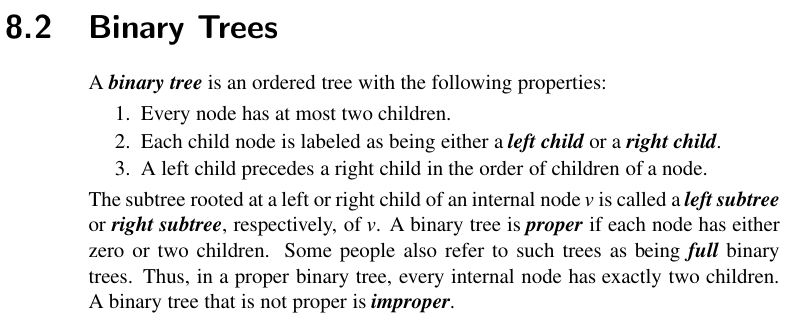
\includegraphics[width=0.7\linewidth]{Immagini/BinaryTree.png}
    \caption{Binary Tree}
\end{figure}

\subsubsection{Binary Tree - Abstract Data Type}

\begin{figure}[H]
    \centering
    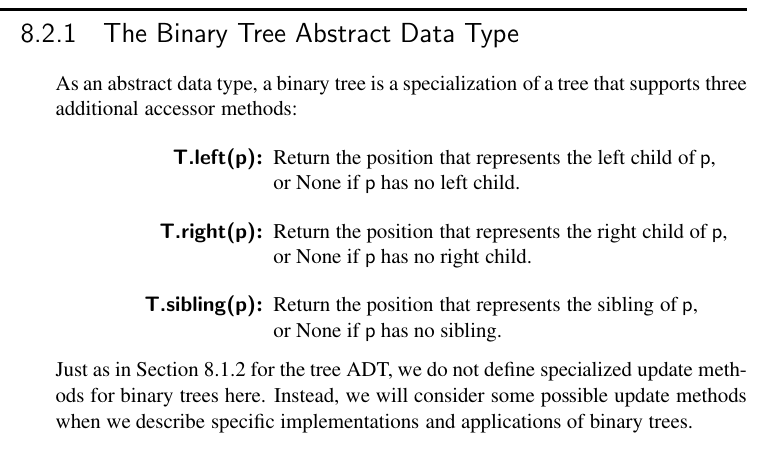
\includegraphics[width=0.7\linewidth]{Immagini/BinaryTreeADT.png}
    \caption{Binary Tree ADT}
\end{figure}

\subsubsection{Properties of Binary Trees}

\begin{figure}[H]
    \centering
    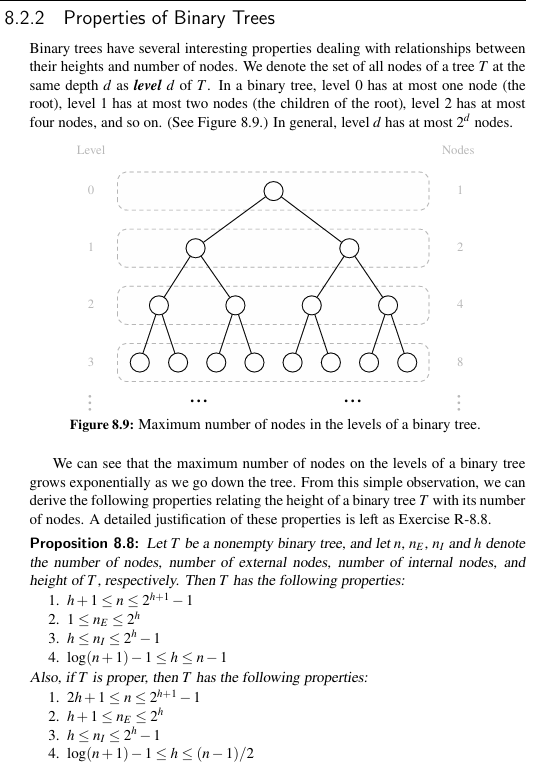
\includegraphics[width=0.7\linewidth]{Immagini/BinaryTreesProperties.png}
    \caption{Binary Tree Properties}
\end{figure}


\begin{figure}[H]
    \centering
    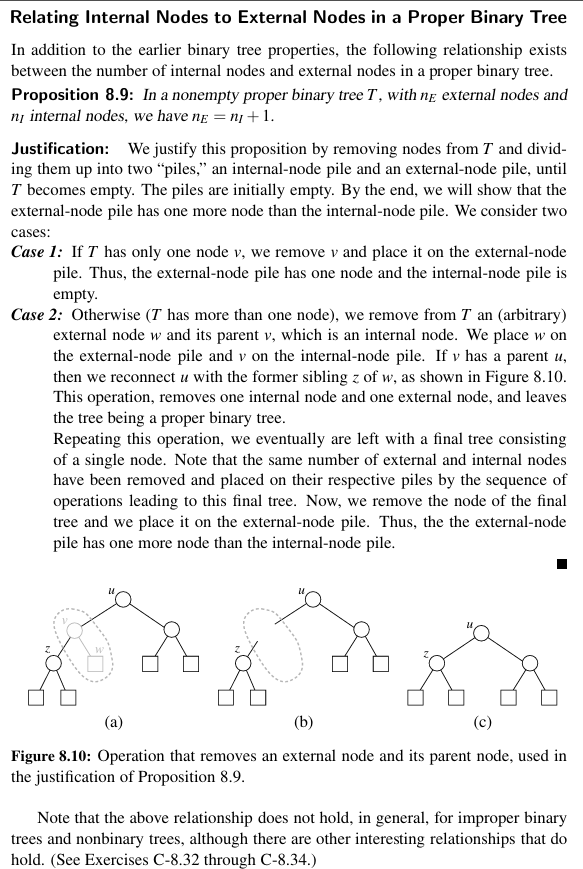
\includegraphics[width=0.7\linewidth]{Immagini/BinaryTreesProperties2.png}
    \caption{Proepr Binary Tree Properties}
\end{figure}

\subsection{General Tree Traversal}
\subsubsection{Preorder e Postorder}
\begin{figure}[H]
    \centering
    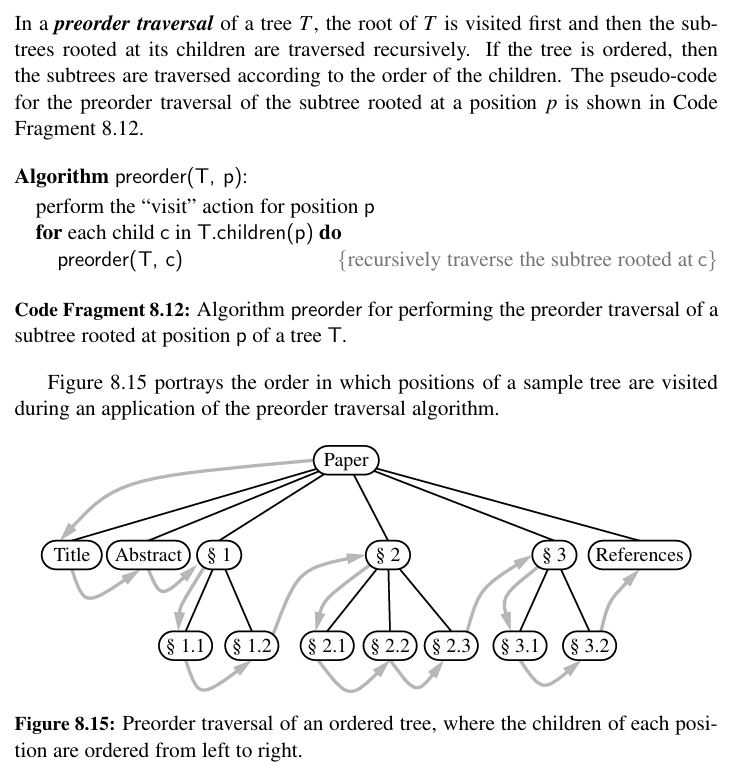
\includegraphics[width=0.7\linewidth]{Immagini/PreorderTraversal.png}
    \caption{Preorder General Tree Traversal}
\end{figure}

\begin{figure}[H]
    \centering
    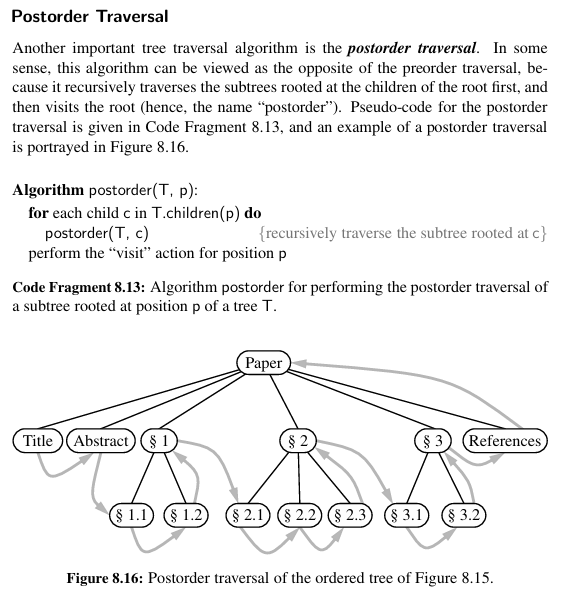
\includegraphics[width=0.7\linewidth]{Immagini/PostorderTraversal.png}
    \caption{Postorder General Tree Traversal}
\end{figure}

\paragraph[H]{Running Time Analysis}
Runtime Analysis di Preorder e Postorder General Tree Traversal
\begin{figure}[H]
    \centering
    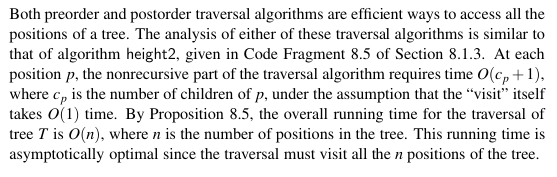
\includegraphics[width=0.7\linewidth]{Immagini/RuntimeAnalysis.png}
    \caption{Running Time Analysis di Postorder e Preorder General Tree Traversal}
\end{figure}

\subsubsection{Breadth-First Tree Traversal}

\begin{figure}[H]
    \centering
    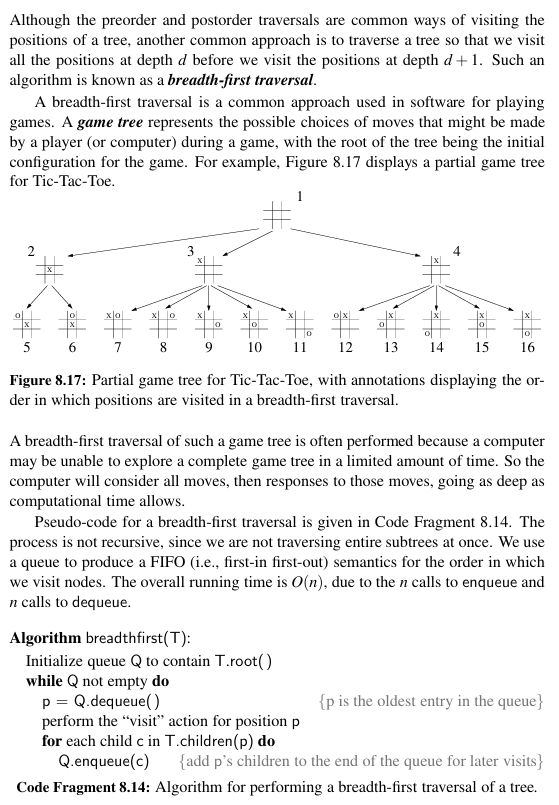
\includegraphics[width=0.7\linewidth]{Immagini/BreadthFirstTrav.png}
    \caption{Breadth-First General Tree Traversal}
\end{figure}

\subsubsection{Inorder Traversal}

\begin{figure}[H]
    \centering
    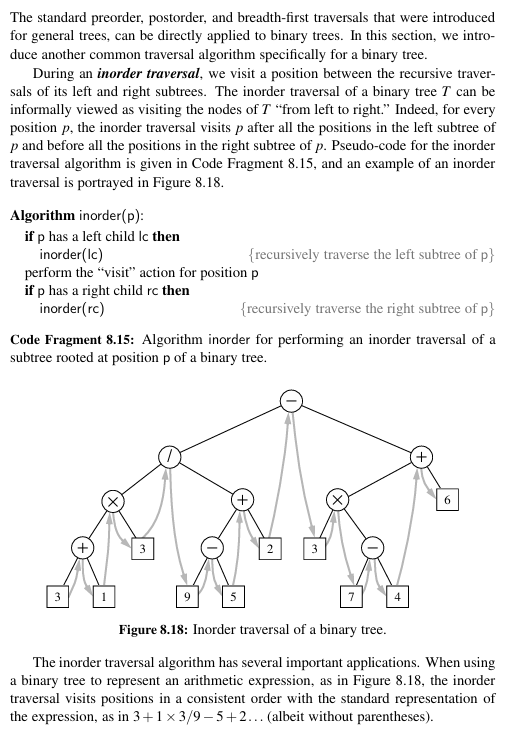
\includegraphics[width=0.7\linewidth]{Immagini/InorderTraversal.png}
    \caption{Inorder General Tree Traversal}
\end{figure}

\subsubsection{Tree Traversal in Python}

\begin{figure}[H]
    \centering
    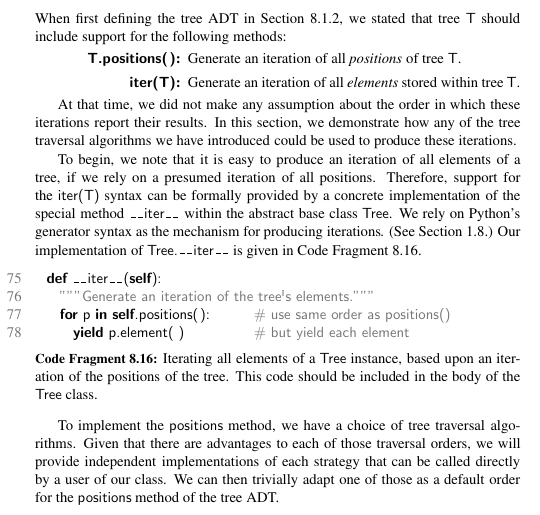
\includegraphics[width=0.7\linewidth]{Immagini/TreeTravPython.png}
    \caption{Tree Traversal in Python}
\end{figure}

\paragraph{Preorder in Python}
Preorder in Python
\begin{figure}[H]
    \centering
    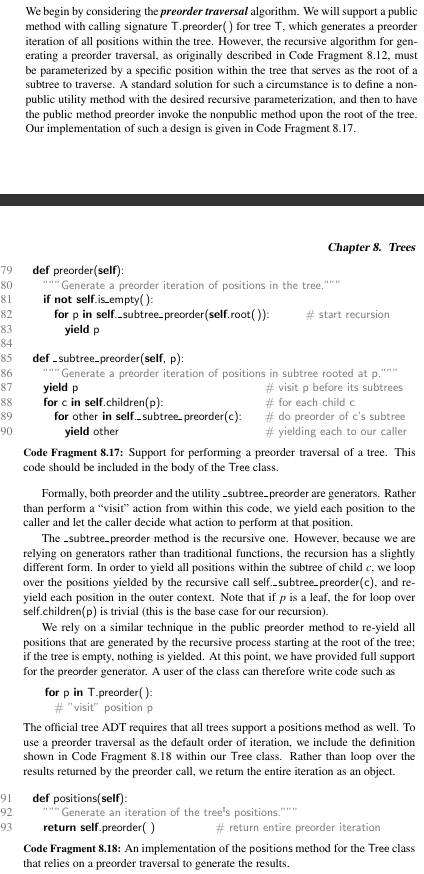
\includegraphics[width=0.7\linewidth]{Immagini/PreorderPython.png}
    \caption{Preorder in Python}
\end{figure}

\paragraph{Postorder in Python}
Postorder in Python
\begin{figure}[H]
    \centering
    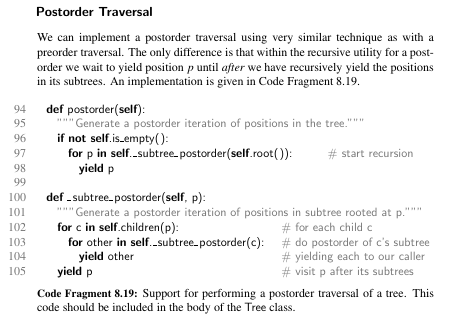
\includegraphics[width=0.7\linewidth]{Immagini/PostorderPython.png}
    \caption{Postorder in Python}
\end{figure}

\paragraph{Breadth-First in Python}
Breadth-First in Python
\begin{figure}[H]
    \centering
    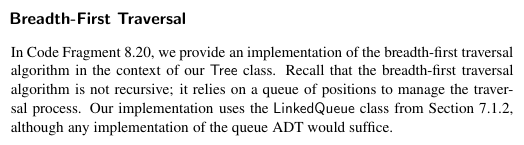
\includegraphics[width=0.7\linewidth]{Immagini/BreadthFirstPython.png}
    \caption{Breadth-First in Python}
\end{figure}

\paragraph{Inoredr in Python}
Inorder in Python
\begin{figure}[H]
    \centering
    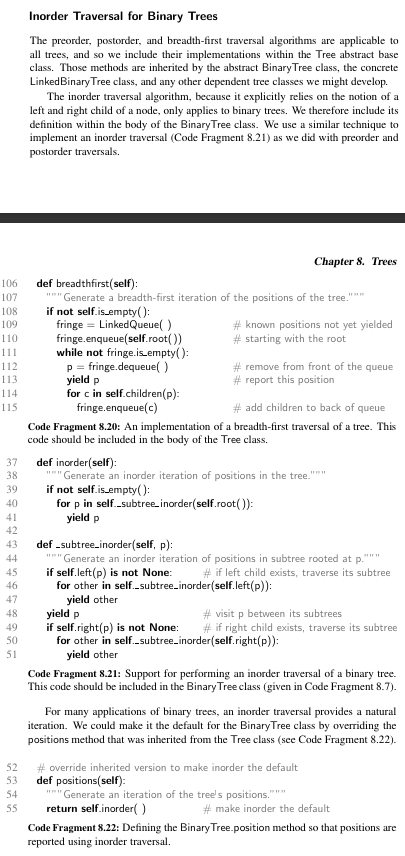
\includegraphics[width=0.7\linewidth]{Immagini/InorderPython.png}
    \caption{Inorder in Python}
\end{figure}





\end{document}